\documentclass[../main.tex]{subfiles}

\begin{document}

\section{Glossary}
\begin{itemize}
  \item Image classification: assign a class label to an image
  \item Object localization: draw a bounding box around one or more objects in an image
  \item Object detection: draw bounding box and assign a label
  \item Object segmentation
  \item Object recognition
\end{itemize}

\section{Datasets}
\begin{itemize}
  \item CalTech-101
  \item VOC-2012
  \item ILSVRC-2013
  \item ImageNet
\end{itemize}

\section{Convolutional Networks}
\begin{itemize}
  \item Convolution layers
  \item Pooling layers
  \item Fully-connected layers
  \item Filters
  \item Stride
  \item BatchNorm
  \item Activation functions
\end{itemize}

\section{CNN Architectures}
\begin{itemize}
  \item ImageNet Classification Challenge
  \item AlexNet
  \begin{itemize}
    \item 227 x 227 inputs
    \item 5 convolutional layers
    \item Max pooling
    \item 3 fully-connected layers
    \item ReLU nonlinearities
    \item 61 million parameters total
  \end{itemize}
  \begin{itemize}
    \item Most memory usage is in the early convolution layers
    \item Nearly all the parameters are from the fully-connected layers
    \item Most floating-point ops occur in convolution layer
  \end{itemize}
  \item VGG
  \begin{itemize}
    \item Enabled training deeper networks
    \item Established standard network design patterns
    \item Design rules:
    \begin{itemize}
      \item All conv are 3x3 stride 1 pad 1
      \item All max pool are 2x2 stride 2
      \item After pool, double the \# of channels
    \end{itemize}
    \item Notes: 2 3x3 conv has the same receptive field as a single 5x5 conv, but fewer parameters and less computation!
    \item VGG-16 total: 138 million parameters
  \end{itemize}
  \item GoogleLeNet
  \begin{itemize}
    \item Many innovations for efficiency: reduce parameters, memory usage, and computation
    \item Stem network: aggressively downsample input from the start
    \item Inception module: local unit with parallel branches, use 1x1 bottleneck to reduce channel before conv
    \item No FC layers at the end
    \item Uses global average pooling to collapse spatial dimensions and one linear layer
    \item Hack to overcome deepness of network, use "auxillary classifier" at intermediate points in network
    \item This work was before BatchNorm!
  \end{itemize}
  \item ResNet
  \begin{itemize}
    \item 152 layers!
    \item Change network so learning identity function with extra layers is easy
    \item Able to train very deep networks
    \begin{figure}[h]
      \caption{Residual Block}
      \centering
      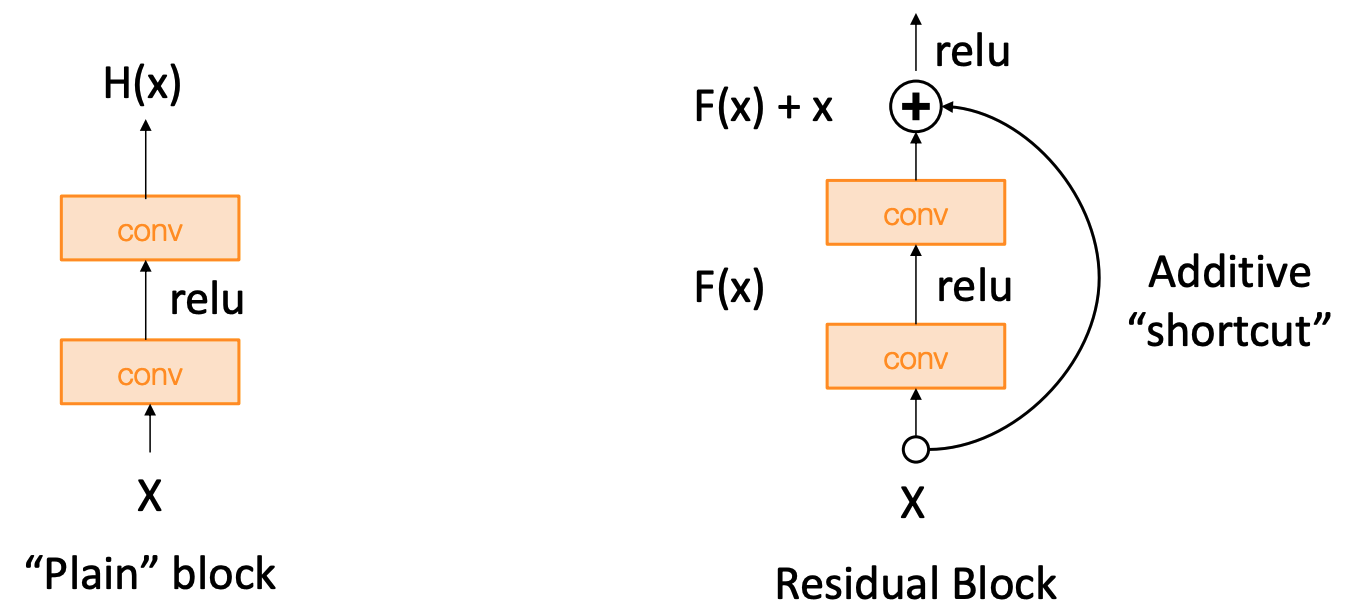
\includegraphics[width=0.5\textwidth]{../imgs/residual_block.png}
    \end{figure}
  \end{itemize}
  \item Densely Connected Neural Networks
  \begin{itemize}
    \item Each layer is connected to every other layer in feedforward
    \item
    \begin{figure}[h]
      \caption{Dense Block}
      \centering
      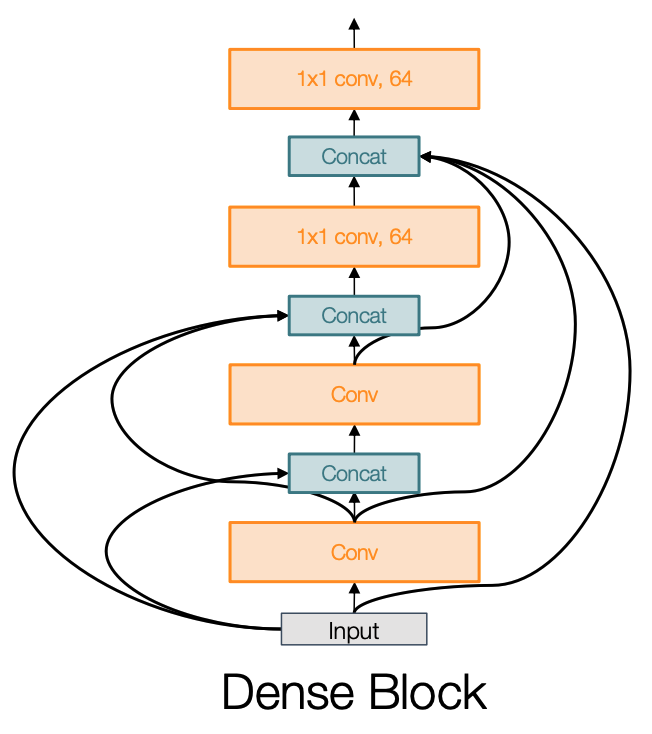
\includegraphics[width=0.3\textwidth]{../imgs/dense_block.png}
    \end{figure}
  \end{itemize}
  \item Tiny networks
  \begin{itemize}
    \item MobileNet
    \item ShuffleNet
  \end{itemize}
  \item Neural Architecture Search
  \begin{itemize}
    \item Automate searching for efficient network architectures
    \item A network outputs network architectures
    \item The controller generates child networks and trains them
    \item After training a batch of child networks, make gradient step on controller network
    \item VERY EXPENSIVE! Trained 800 GPUs for 28 days
  \end{itemize}
\end{itemize}

\section{Recurrent Networks}
\begin{itemize}
  \item Recurrent Neural Networks
  \begin{itemize}
    \item useful for processing sequences with inputs
    \item one-to-one, one-to-many (image captioning), many-to-one (video classification), many-to-many (machine translation)
    \item Key idea is that RNN have an "internal state" that is updated as a sequence is processed
    \begin{equation*}
      h_{t} = f_{W}(h_{t-1}, x_{t})
    \end{equation*}
    \begin{conditions}
      x_{t} & input vector \\
      h_{t} & new state \\
      f_{W} & function with parameter W \\
    \end{conditions}
    \item Vanilla RNN
    \begin{align*}
      h_{t} &= \text{tanh}(W_{hh}h_{t-1} + W_{xh}x_{t} + b_{h}) \\
      y_{t} &= W_{hy}h_{t} + b_{y}
    \end{align*}
    \item Reuse weight matrix at every timestep
    \item Backpropagation through time
    \item RNN forwards the entire sequence to compute loss and then backward through the entire sequence to compute gradients
    \item Language modeling - generating Shakespeare poems, generating code, etc
    \item Image captioning - first run CNN on image and feed output from FC-4096 into the RNN along with captions
    \item Backprop results in exploding / vanishing gradients
    \item For exploding gradients, we can use gradient clipping to scale the gradient if norm is too big
    \item For vanishing gradients, we need to change the RNN architecture
  \end{itemize}
  \item Long-short Term Memory
  \begin{align*}
    i_{t} &= \sigma(W_{hh}h_{t-1} + W_{xh}x_{t} + b_{h}) \\
    f_{t} &= \sigma(W_{hh}h_{t-1} + W_{xh}x_{t} + b_{h}) \\
    o_{t} &= \sigma(W_{hh}h_{t-1} + W_{xh}x_{t} + b_{h}) \\
    g_{t} &= \text{tanh}(W_{hh}h_{t-1} + W_{xh}x_{t} + b_{h}) \\
    c_{t} &= f_{t} \odot c_{t-1} + i_{t} \odot{g_{t}}\\
    h_{t} &= o_{t} \odot \text{tanh}(c_{t})
  \end{align*}
  \begin{conditions}
    i & input gate: whether to write to cell \\
    f & forget gate: whether to erase cell \\
    o & output gate: how much to reveal cell \\
    g & gate gate (?): how much to write in a cell \\
  \end{conditions}
  \item Backpropagation from $c_{t}$ to $c_{t-1}$ is only elementwise multiplication by $f$, does not depend on matrix multiply by $W$
  \begin{figure}[h]
      \caption{LSTM Cell}
      \centering
      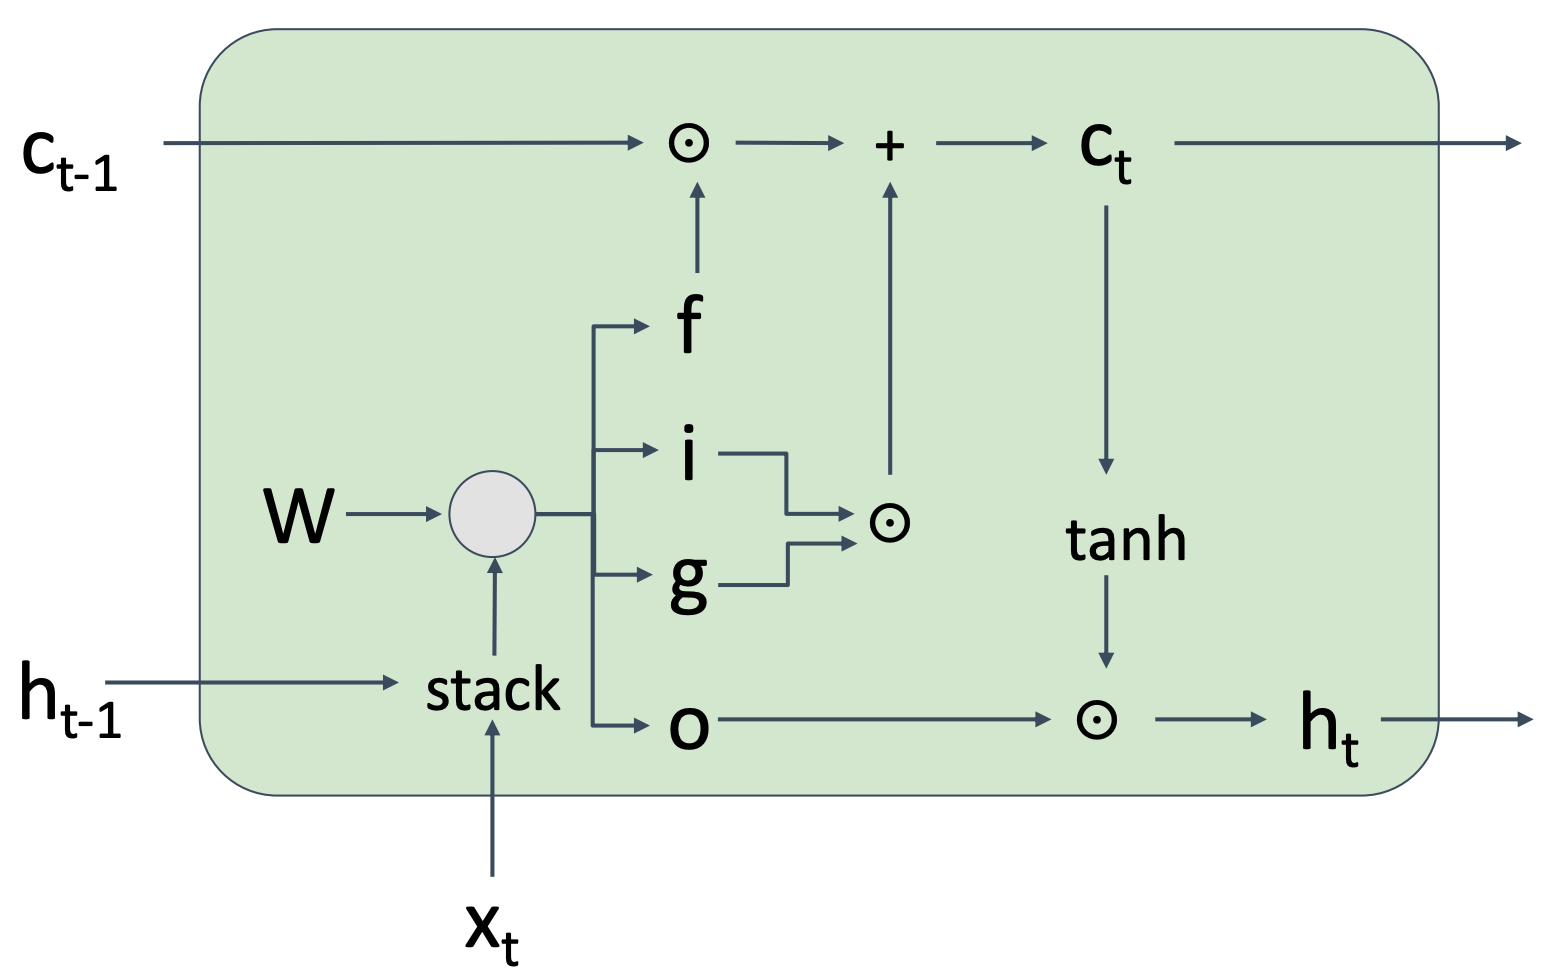
\includegraphics[width=0.5\textwidth]{../imgs/lstm_cell.png}
    \end{figure}
  \item Gated Recurrent Units
  \begin{itemize}
    \item
  \end{itemize}
\end{itemize}

\section{RCNN and variants}
\begin{itemize}
  \item \cite{rcnn}
  \item Region Proposal
  \begin{itemize}
    \item Generate and extract category independent region proposals, candidate bounding boxes
    \item Use CV technique called "selective search"
    \item AlexNet
  \end{itemize}

  \item Feature Extractor
  \begin{itemize}
    \item Extract feature from each candidate region
  \end{itemize}

  \item Classifier
  \begin{itemize}
    \item Classify feature as one of the know classes
  \end{itemize}

\end{itemize}

\subsection{Other popular architectures}

\section{Detection}
\subsection{Single-stage detectors}
\subsection{Two-stage detectors}

\section{Segmentation}
\subsection{Semantic segmentation}
\subsection{Instance segmentation}
\subsection{Keypoint estimation}

\section{Domain Adaptation}

\section{3D}
\subsection{Representations}
\begin{itemize}
  \begin{figure}[h]
      \caption{3D shape representations}
      \centering
      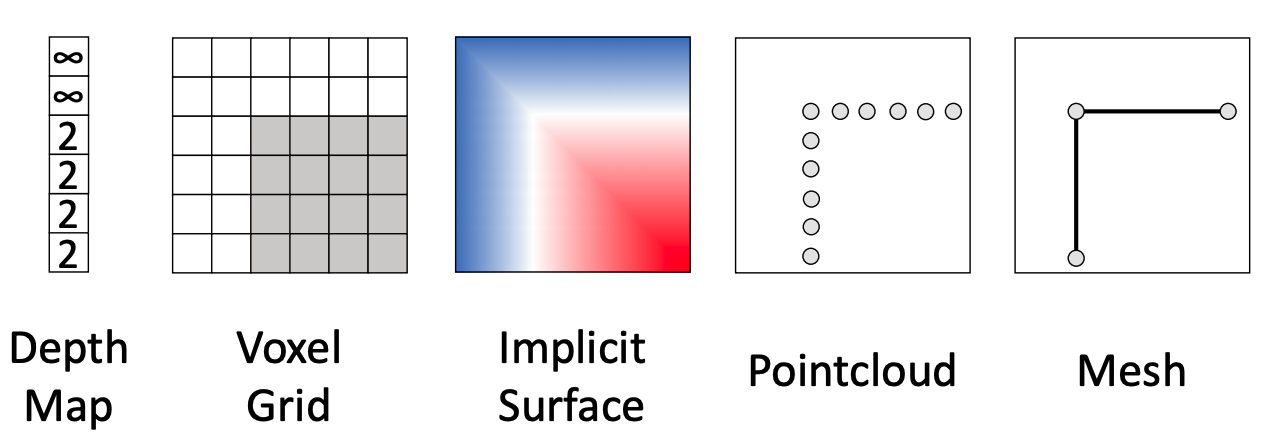
\includegraphics[width=0.5\textwidth]{../imgs/3d_representations.png}
  \end{figure}

  \item Depth Map
  \begin{itemize}
    \item Distance from camera to object into the world at each pixel
    \item Often combined with RGB image = RGB-D image (2.5D)
    \item Can't capture occuluded areas
    \item e.g. Microsoft Kinect and new IPhone-12 sensors
    \item Task: predicting depth map from RGB image
    \item Scale / depth ambiguity
  \end{itemize}
  \item Surface Normals
  \begin{itemize}
    \item Normal vector to object in world at pixel
    \item Useful for robotics applications such as grasping objects
    \item Can get ground-truth surface normal using synthetic data or multiview 3D reconstruction
    \item Predict surface normal representation, loss: penalizes the angle between vectors
  \end{itemize}
  \item Voxel Grid
  \begin{itemize}
    \item A shape is a V x V x V grid of binary occupancies, any type of data can be stored in a cell of voxel representation
    \item Like segmentation mask in 3D rather than 2D
    \item Need high spatial resolution to capture fine-grain objects
    \item Scaling to high resolutions is nontrivial, computationally expensive
    \item Process these with 3D convolution
    \item Generating voxel shapes using 3D convolution, flatten 2D features and convert into 3D feature
    \item Predict per voxel and take loss per voxel
    \item Memory usage scales cubically, not tractable
    \item Oct-Trees for scaling voxels with heterogenous resolutions
  \end{itemize}

  \item Implicit Surfaces
  \begin{itemize}
    \item Learn function to classify arbitrary 3D points as inside / outside the shape or predict some sort of data
    \item The surface of the 3D object is the level set
    \item $o: \mbb{R}^{3} \rightarrow \{0,1\}$
  \end{itemize}

  \item Pointclouds
  \begin{itemize}
    \item Represent shape as set of points in 3D space
    \item Can represent fine structures without huge \# of points
    \item Requires new architectures / losses
    \item Don't explicitly represent the surface! Need some postprocessing to get a mesh representation
    \item PointNet: run MLP on each point in the cloud to generate per-point feature vector $\rightarrow$ max pooling then a fully-connected vector
  \end{itemize}

  \item Triangle Mesh
  \begin{itemize}
    \item Commonly used in computer graphics
    \item Represent 3D shape as a set of triangles
    \item Adaptive: can reprsent flat surfaces very efficiently, allocate more faces with fine detail
    \item Can interpolate data on vertices over whole surfaces like RGB color, normal vector
    \item Pixel2Mesh: single RGB image $\rightarrow$ triangle mesh
  \end{itemize}

\end{itemize}

\subsection{Depth estimation}
\subsection{3D shape prediction}
\subsection{Voxels and pointclouds}
\subsection{Structure from Motion}
\subsection{View Synthesis}
\subsection{Differentiable Graphics}

\section{Dataset biases}

\section{Vision and language}

\section{Vision and sound}

\section{Attention for vision}

\end{document}